\section{Concurrency}

\subsection{Motivation}
\begin{itemize}
  \item Praktische Programme führen meist mehrere Arbeiten "`gleichzeitig"' aus. 
  \item Diese Nebenläufigkeit kann implementiert werden durch\ldots
  \begin{itemize}
    \item Quasi-Parallelität durch Betriebssystem $\rightarrow$ Synchronisation
    nötig, da auf gemeinsame Ressourcen zugegriffen wird
    \item Echte Parallelität durch Mehrprozessorsystem
  \end{itemize}
\end{itemize}
Richtwert: Aufgaben welche länger als 100ms dauern, sollten in den Worker-Thread ausgelagert werden.

\subsection{Parallel VS Concurrent computing}
\begin{multicols}{2}
  Parallel Computing:
  \begin{itemize}
    \item Ausf\"uhrung von verschiedenen Aufgaben werden zur selben Zeit erledigt.
    \item Nur bei Multiprozessor-Controller m\"oglich
  \end{itemize}
\vfill\null
\columnbreak
  Concurrent Computing
  \begin{itemize}
    \item Ausf\"uhrung scheint nur parallel abzulaufen
    \item Verschiedene Aufgaben werden bestimmte Zeitpunkte durch Scheduler zugeteilt
    \item Nur eine Aufgabe wird im Moment bearbeitet
    \item Realisierbar mit single- und multicore- Prozessoren
  \end{itemize}
\end{multicols}

\textbf{Nachteile von Nebenläufigkeit}
\begin{itemize}
  \item  Concurrency (mit Prozessen, Tasks, Threads) kostet immer \ldots
  \begin{itemize}
    \item \ldots Stack
    \item \ldots Kontext switch
    \item \ldots Zugriffe auf gemeinsame Ressourcen muss synchronisiert werden.
  \end{itemize}
  \item  Komplexität steigt. Sequentielle Programme sind einfacher zu verstehen als parallele.
\end{itemize}
Concurrency nur dann einsetzen, wenn wirklich ein nutzen vorhanden ist.

\subsection{Threads in CSharp \buch{p.7}}
Prozesse und Threads aus OS-Sicht:\\
\begin{center}
{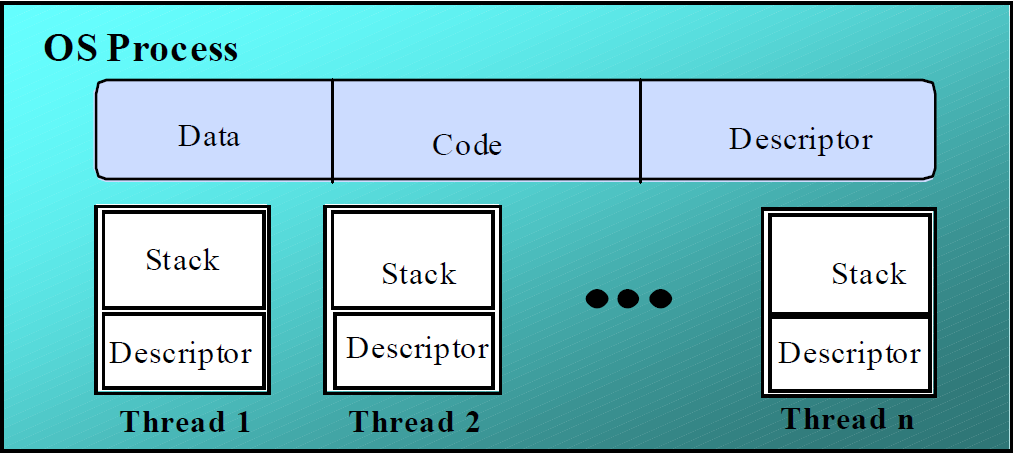
\includegraphics[width=0.5\textwidth]{images/Concurrency/ProzesseUndThreads.png}}
\end{center}
\begin{itemize}
  \item Prozess (heavyweight process):
  \begin{itemize}
    \item Code
    \item Daten
    \item Deskriptor zur Verwaltung des Prozesses durch OS (PCB, Process
    Control Block)
  \end{itemize}
  \item Thread (lightweight process):
  \begin{itemize}
    \item Teil eines Prozesses
    \item Gemeinsamer Adressraum
    \item Gemeinsame Nutzung anderer System-Ressourcen
    \item Pro Thread: Code, Stack, Deskriptor
  \end{itemize}
\end{itemize}
Ein Thread unterscheidet sich zu einem Prozess folgendermassen:\\
Man beachte: Ein Thread ist Teil eines Prozesses, das bedeutet, alles was ein
Thread inne hat, hat ein Prozess auch inne (aber NICHT umgekehrt)!\\
\begin{centering}
  \begin{tabular}{l | l}
    \hline
    \hline
    Pro Prozess vorhanden & Pro Thread vorhanden\\
    \hline
    \hline
    Adressraum & Programmzähler\\
    \hline
    Globale Variabeln & Register\\
    \hline
    Geöffnete Dateien & Stapel(Stack)\\ 
    \hline
    Kindprozesse & Zustand\\
    \hline 
    Pendente Alarme & \\
    \hline 
    Signale und Signalbehandlungsroutinen &\\
    \hline
    Buchhaltungsinformationen
  \end{tabular}
\end{centering}\\

Quasiparallelität:\\
Prozesse/Threads können folgende Zustände und Übergänge erfahren: 
\begin{center}
{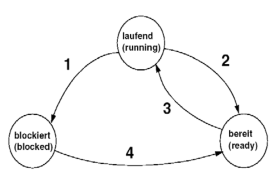
\includegraphics[width=0.5\textwidth]{images/Concurrency/Prozesszustaende.png}}
%\label{Fig: Schlechtes Beispiel für Modularisierung}
\end{center}
